% imports
\begin{figure*}
\centering
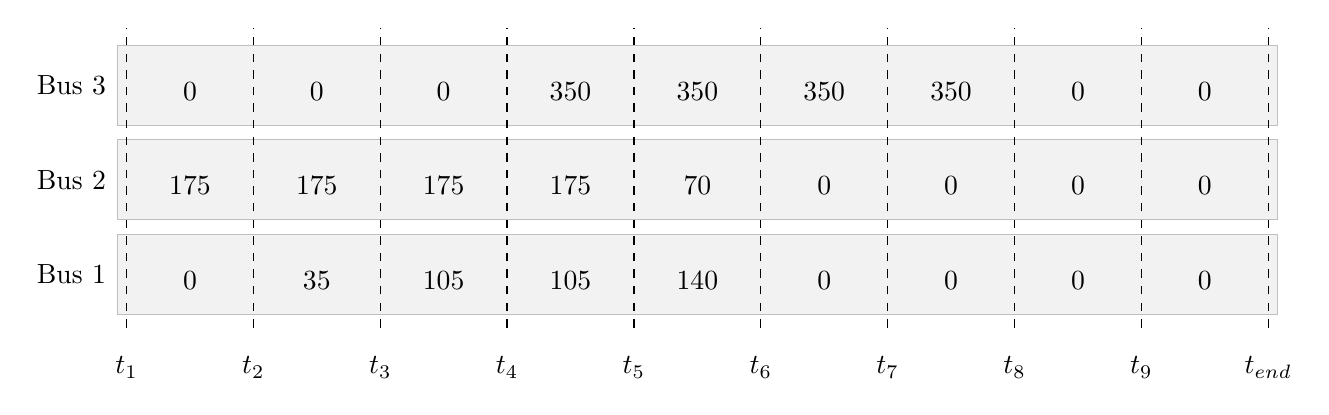
\begin{tikzpicture}
	\node[rectangle, draw=gray!50, fill=gray!10, minimum width=5.8in, minimum height=0.4in](bus1Box) at (7.75,0.8){};
	\node(bus1BoxLabel) at (-0.2, 0.8){Bus 1}; 
	
	\node[rectangle, draw=gray!50, fill=gray!10, minimum width=5.8in, minimum height=0.4in](bus2Box) at (7.75,2){};
	\node(bus1BoxLabel) at (-0.2, 2.0){Bus 2};
	
	\node[rectangle, draw=gray!50, fill=gray!10, minimum width=5.8in, minimum height=0.4in](bus3Box) at (7.75,3.2){};
	\node(bus1BoxLabel) at (-0.2, 3.2){Bus 3};
	
	\foreach \curLab/\preLab[count=\c, evaluate=\c as \pos using {0.5 + (\c - 1)*14.5/9}] in {t_1/t_1, t_2/t_1, t_3/t_2, t_4/t_3, t_5/t_4, t_6/t_7, t_7/t_6, t_8/t_7, t_9/t_8, t_{end}/t_9}
	{
		\node[label=below:$\curLab$](b\c) at (\pos, 0){};
		\node(t) at (\pos, 3.8){};
		\draw[dashed, line width=0.5pt] (b\c.north) -- (t.north); 
		\ifnum\c>1 
			\node(b1Curr) at (\pos, 0.8 - 0.2){};
			\node(b2Curr) at (\pos, 2.0 - 0.2){};
			\node(b3Curr) at (\pos, 3.2 - 0.2){};
			\path(b1Prev.east) -- node(node1\c)[midway, above]{}(b1Curr.west);
			\path(b2Prev.east) -- node(node2\c)[midway, above]{}(b2Curr.west);
			\path(b3Prev.east) -- node(node3\c)[midway, above]{}(b3Curr.west);	
		\fi
			\node(b1Prev) at (\pos, 0.8 - 0.2){};
			\node(b2Prev) at (\pos, 2.0 - 0.2){};
			\node(b3Prev) at (\pos, 3.2 - 0.2){};	
	}
	\path (b9.south) -- node[midway, below=0.1in]{$\hdots$}(b10.south);
	\node at (node12.center){0};
	\node at (node13.center){35};
	\node at (node14.center){105};
	\node at (node15.center){105};
	\node at (node16.center){140};
	\node at (node17.center){0};
	\node at (node18.center){0};
	\node at (node19.center){0};
	\node at (node110.center){0};
	\node at (node22.center){175};
	\node at (node23.center){175};
	\node at (node24.center){175};
	\node at (node25.center){175};
	\node at (node26.center){70};
	\node at (node27.center){0};
	\node at (node28.center){0};
	\node at (node29.center){0};
	\node at (node210.center){0};
	\node at (node32.center){0};
	\node at (node33.center){0};
	\node at (node34.center){0};
	\node at (node35.center){350};
	\node at (node36.center){350};
	\node at (node37.center){350};
	\node at (node38.center){350};
	\node at (node39.center){0};
	\node at (node310.center){0};

\end{tikzpicture}
\caption{An example solution to a 3-bus, 2-charger scenario from the first QP}
\label{fig:solutionExample}
\end{figure*}

\begin{figure*}
\centering
\scalebox{0.8}{
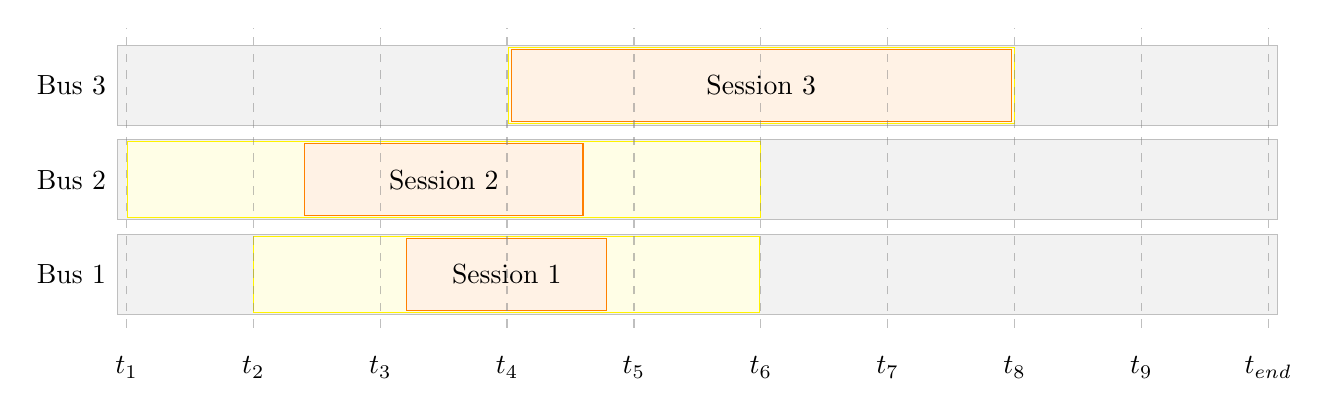
\begin{tikzpicture}
	\node[rectangle, draw=gray!50, fill=gray!10, minimum width=5.8in, minimum height=0.4in](bus1Box) at (7.75,0.8){};
	\node(bus1BoxLabel) at (-0.2, 0.8){Bus 1}; 
	\node[rectangle, draw=yellow!100, fill=yellow!10, minimum width=2.53in, minimum height=0.38in](charge11) at (5.33, 0.8){};
	\node[rectangle, draw=orange!100, fill=orange!10, minimum width=1in, minimum height=0.36in](charge111) at (5.33, 0.8){Session 1};

	\node[rectangle, draw=gray!50, fill=gray!10, minimum width=5.8in, minimum height=0.4in](bus2Box) at (7.75,2){};
	\node(bus1BoxLabel) at (-0.2, 2.0){Bus 2};
	\node[rectangle, draw=yellow!100, fill=yellow!10, minimum width=3.1625in, minimum height=0.38in](charge11) at (4.53, 2){};
	\node[rectangle, draw=orange!100, fill=orange!10, minimum width=1.3915in, minimum height=0.36in](charge111) at (4.53, 2){Session 2};
	
	\node[rectangle, draw=gray!50, fill=gray!10, minimum width=5.8in, minimum height=0.4in](bus3Box) at (7.75,3.2){};
	\node(bus1BoxLabel) at (-0.2, 3.2){Bus 3}; 
	\node[rectangle, draw=yellow!100, fill=yellow!10, minimum width=2.53in, minimum height=0.38in](charge11) at (8.56, 3.2){};
	\node[rectangle, draw=orange!100, fill=orange!10, minimum width=2.50in, minimum height=0.36in](charge111) at (8.56, 3.2){Session 3};


	\foreach \curLab/\preLab[count=\c, evaluate=\c as \pos using {0.5 + (\c - 1)*14.5/9}] in {t_1/t_1, t_2/t_1, t_3/t_2, t_4/t_3, t_5/t_4, t_6/t_7, t_7/t_6, t_8/t_7, t_9/t_8, t_{end}/t_9}
		{
			\node[label=below:$\curLab$](b\c) at (\pos, 0){};
			\node(t) at (\pos, 3.8){};
			\draw[dashed, line width=0.5pt, black!50, opacity=0.5] (b\c.north) -- (t.north); 
		}
		\path (b9.south) -- node[midway, below=0.1in]{$\hdots$}(b10.south); 
\end{tikzpicture}}
\caption{Demonstrates how results from $p_4$ can be reexpressed in terms of continuous variables} 
\label{fig:refactorExample}
\end{figure*}



\begin{figure*}
\centering
\scalebox{0.8}{
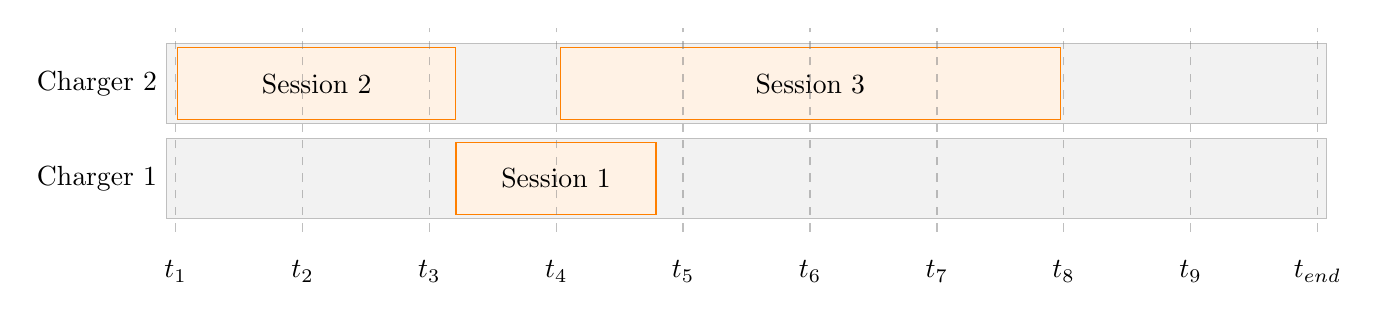
\begin{tikzpicture}
	\node[rectangle, draw=gray!50, fill=gray!10, minimum width=5.8in, minimum height=0.4in](bus1Box) at (7.75,0.8){};
	\node(bus1BoxLabel) at (-0.5, 0.8){Charger 1}; 

	\node[rectangle, draw=gray!50, fill=gray!10, minimum width=5.8in, minimum height=0.4in](bus2Box) at (7.75,2){};
	\node(bus1BoxLabel) at (-0.5, 2.0){Charger 2};
	\node[rectangle, draw=orange!100, fill=orange!10, minimum width=1.3915in, minimum height=0.36in](charge111) at (2.29, 2){Session 2}; 
	\node[rectangle, draw=orange!100, fill=orange!10, minimum width=1in, minimum height=0.36in](charge111) at (5.33, 0.8){Session 1};
	\node[rectangle, draw=orange!100, fill=orange!10, minimum width=2.50in, minimum height=0.36in](charge111) at (8.56, 2){Session 3};


	\foreach \curLab/\preLab[count=\c, evaluate=\c as \pos using {0.5 + (\c - 1)*14.5/9}] in {t_1/t_1, t_2/t_1, t_3/t_2, t_4/t_3, t_5/t_4, t_6/t_7, t_7/t_6, t_8/t_7, t_9/t_8, t_{end}/t_9}
		{
			\node[label=below:$\curLab$](b\c) at (\pos, 0){};
			\node(t) at (\pos, 2.58){};
			\draw[dashed, line width=0.5pt, black!50, opacity=0.5] (b\c.north) -- (t.north); 
		}
		\path (b9.south) -- node[midway, below=0.1in]{$\hdots$}(b10.south); 
\end{tikzpicture}}
\caption{Demonstrates the solution to $p_5$}
\label{fig:secondSolutionExample}
\end{figure*}



\begin{figure*}
\centering
\scalebox{0.8}{
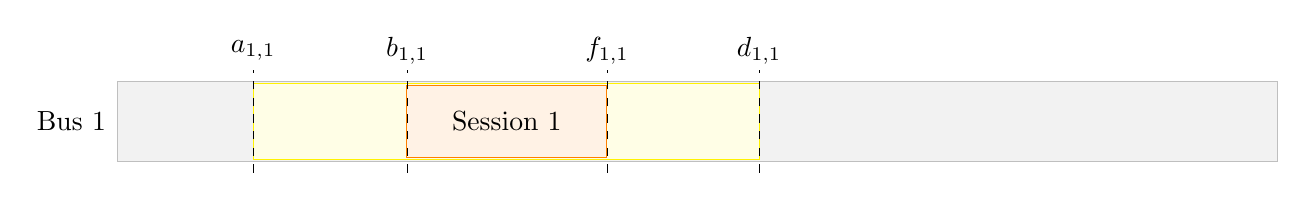
\begin{tikzpicture}
	\node[rectangle, draw=gray!50, fill=gray!10, minimum width=5.8in, minimum height=0.4in](bus1Box) at (7.75,0.8){};
	\node(bus1BoxLabel) at (-0.2, 0.8){Bus 1}; 
	\node[rectangle, draw=yellow!100, fill=yellow!10, minimum width=2.53in, minimum height=0.38in](charge11) at (5.33, 0.8){};
	\node[rectangle, draw=orange!100, fill=orange!10, minimum width=1in, minimum height=0.36in](charge111) at (5.33, 0.8){Session 1}; 
	\draw[dashed] (0.83in,0.15) -- (0.83in,1.45);
	\node at (0.83in,1.7){$a_{1,1}$};
	\draw[dashed] (3.36in, 0.15) -- (3.36in, 1.45);
	\node at (3.36in,1.7){$d_{1,1}$};
	\draw[dashed] (1.6in, 0.15) -- (1.6in, 1.45);
	\node at (1.6in,1.7){$b_{1,1}$};
	\draw[dashed] (2.6in, 0.15) -- (2.6in, 1.45);
	\node at (2.6in,1.7){$f_{1,1}$};
\end{tikzpicture}}
\caption{Gives variables of optimization for $p_5$}
\label{fig:secondProgramVars}
\end{figure*} 


\section{$p_5$: Charger Assignment\label{sec:chargerAssignment}}
The results from $p_4$ give a general estimate of how much and when buses should charge, however we must still address two primary issues. The first is defining concrete start and stop times for each charge session. The second is limiting the charge sessions to a finite number of chargers. 
\par Consider a solution to a three bus, two charger scenario given in Fig. \ref{fig:solutionExample}.
Note that there appears to be three buses charging at the same time from $t_5$ to $t_6$ even though there are only two chargers.  We can reformulate this solution in terms of continuous start and stop variables and a variable charge rate so that the {\it duration} of each charge session may be relaxed. The objective is to store the given energy in the corresponding bus within the given charge interval.  
\par Note how few of the charge sessions utilize the chargers to full capacity. This implies that there exists a smaller charge window in which equivalent power can be delivered. This allow us to use the charge durations from the solution from Fig. \ref{fig:solutionExample} as bounds on {\it allowable} charge windows instead of absolute truth. 
\par An example of how Fig. \ref{fig:solutionExample} may be reformulated is given in Fig. \ref{fig:refactorExample}. Note how the actual charge sessions don't necessarily need to take up all the time they were initially allocated in the first solution and that these times can fluctuate if the average charge rate is less than the maximum charger capacity. In this example, we assume a maximum charge capacity of 350kW.  
\par Note how the third charge session does have to be exactly where it was scheduled because the average is equal to the maximum charge rate.
If we examin just the schedule for Bus 1, we note that there are four essential variables for the corresponding charge session: $a(i,r)$, $b(i,r)$, $f(i,r)$ and $d(i,r)$ which represent the minimum start time, actual start time, actual end time, and maximum end time respectively. 
\par The problem we must now solve is one of arranging these ``rectangles'' such that each one is larger than it's minimum width (or charge time).  We must also account for the number of chargers. It can be helpful to view the problem as a bin packing problem, where each session must fit within the ``swim lane'' of a charger.  For example, taking the charge sessions given in Fig. \ref{fig:refactorExample} and arranging them so that there is no overlap between sessions will yield a valid solution as shown in Fig. \ref{fig:secondSolutionExample}.
\par From Fig. \ref{fig:secondProgramVars}, we know that $a(i,r), b(i,r),f(i,r)$ and $d(i,r)$ must be such that 
\begin{equation}\label{eqn:assignment:eqn1}\begin{aligned}
	a(i,r) \le b(i,r) \\
	b(i,r) \le f(i,r) \\
	f(i,r) \le d(i,r). 	
\end{aligned}\end{equation}
where $a(i,r)$ and $d(i,r)$ are known from the previous optimization problem, and $b(i,r)$ and $f(i,r)$ are optimization variables. 
\par We must differentiate between chargers and so, define $\sigma(i,r,k)$ as a binary selector variable which is one if charger $k$ services bus $i$ for session $r$ and zero otherwise. We know that only one charger can charge each bus at a time. We also know that each charge session {\it must} be serviced, which implies that
\begin{equation}\label{eqn:assignment:eqn2}
	\sum_k \sigma(i,r,k) = 1  \ \forall i,r.
\end{equation}
\par Next, we also know that during each session a certain amount of energy must be transfered from the charger to the battery.  The amount of energy that must be transfered to bus $i$ during session $r$ are given in the solution to $p_4$ and are denoted $e(i,r)$. We can compute a minimum time window from these values by letting 
\begin{equation}\label{eqn:assignment:eqn3}
	w(i,r)_{\text{min}} = \frac{e(i,r)}{p_\text{max}}.
\end{equation}
If we include constraints for a minimum time per session, then the previous expression becomes
\begin{equation*}
	w(i,r)_{\text{min}} = \text{max}\left ( w_{\text{min}}, \frac{e(i,r)}{p_\text{max}} \right )
\end{equation*}
\par Because this is the minimum time window, we must ensure that the difference between the start and stop times is at least this large so that
\begin{equation}\label{eqn:assignment:eqn4}
	f(i,r) - b(i,r) \ge w(i,r) \ \forall i,r.
\end{equation}
\par The final set of constraints deals with contention so that no charger can be scheduled for two sessions that overlap. let $\mathcal{L} = \{(i,r)\times (i',r') \}$ where charge sessions $i,r$ and $i',r'$ have the potential to overlap. Before we can prevent overlap, we must define a binary variable $l(i,r,i',r')$ which is equal to one when session $i,r$ is scheduled before session $i',r'$ and zero otherwise so that
\begin{equation}
	\begin{cases}
		f(i,r) \le b(i',r') & l(i,r,i',r') = 1 \\
		f(i',r') \le b(i',r') & l(i,r,i',r') = 0 
	\end{cases}
\end{equation}
Here we can expand this thought through use of the ``big-M'' technique.  Let $M$ be large. In this case, we can set it equal to the number of seconds in a day. We know what the top constraint must be trivially satisfied when $l(i,r,i',r') = 0$ and the bottom must also when $l(i,r,i',r') = 1$.  This leads to a reformulation so that
\begin{equation*}\begin{aligned}
		f(i,r) - b(i',r') & \le M(1 - l(i,r,i',r')\\
		f(i',r') - b(i,r) & \le l(i,r,i',r')M  
\end{aligned}\end{equation*}
However, this constraint {\it only} needs to hold when sessions $i,r$ and $i',r'$ are scheduled to charge on the same charger or that $\sigma(i,r,k) = \sigma(i',r',k) = 1$. We can reformulate the above constraint to satisfy this condition by letting
\begin{equation}\label{eqn:assignment:eqn5}\begin{aligned}
	f(i,r) - b(i',r') & \le M(3 - \sigma(i,r,k) - \sigma(i',r',k) - l(i,r,i',r')) \\
	f(i',r') - b(i,r) & \le M(2 - \sigma(i,r,k) - \sigma(i',r',k) + l(i,r,i',r'))
\end{aligned}\end{equation}
\par Finally, we desire the schedule to closly match the charge plan from $p_4$, which occures when each charge session matches the durations given in $p_4$ and so we formulated an objective function which minimizes the differences in the given plan and the results from $p_4$ by letting the objective be
\begin{equation}\label{eqn:assignment:eqn6}
	\underset{f,b}{\text{min}} \sum_{i,r}\lVert b(i,r) - a(i,r)\rVert_2^2 + \lVert f(i,r) - d(i,r) \rVert_2^2
\end{equation}
which has the effect of driving each variable to the desired value and more heavily penalizing values that are further from their optimal.
\par Ideally, when $p_5$ is solved to optimality, the chargers are fully utilized. However, optimality for $p_5$ is computationally demanding and scalable solutions may require relaxations in the optimality gap so that time on the chargers is not fully utilized. The next section uses the ordering from $p_5$, but recomputes session start/stop times to better utilize the charger availability even when sub-optimal gaps are given for $p_5$.
\\[0.1in] \begin{tikzpicture}
	\node[rectangle, rounded corners, fill=gray!8, draw=gray!60, minimum width=\columnwidth, minimum height=0.7in] at (0,0)(box){};
	\node at (0,0.2in)(title){\underline{Summary for $p_5$}};
	\node at ($(box.south)!0.6!(title.south)$)(text){$
	\underset{\mathbf{y}}{\text{Min}} \ \eqref{eqn:assignment:eqn6} \ \text{subject to} \ \eqref{eqn:assignment:eqn1} \ \text{--} \ \eqref{eqn:assignment:eqn5}.
$};
\end{tikzpicture} 

\section{$p_6$: Optimizing Charge Schedules\label{sec:optimizingChargeSchedules}}
Many times it is not feasible to compute the optimal set of charge schedules given in the previous sections. As the number of buses and charge sessions becomes large, computing a small-MIPGap solution becomes untractable. Using a large MIPGap resolves issues related to computational complexity, but results in sub-optimal charge-time windows.
\par We compute a more optimal set of charge windows by using the results from $p_5$ to infer charger assignment, and ordering for each charge session. We also know that the optimal solution will expand the charge windows to use any available time where a charger is unused, implying that the ``stop'' time for each session will either be equal to it's buse's departure time, or the start time of the next window which can be expressed as
\begin{equation}\label{eqn:optChargeSchedules:eqn1}
\begin{cases}
	c(s,i,r+1) = c(f,i,r) & c(d,i,r) > c(a,i,r+1)\\[0.08in]
	\begin{aligned}
	c(s,i,r+1) &= c(a,i,r+1) \\
	c(f,i,r) &= c(d,i,r)
	\end{aligned} & c(d,i,r) <= c(a,i,r+1) \\
\end{cases}
\end{equation}
where $c(s,i,r)$ is the start time for charger $i$'s $r^{\text{th}}$ charge session, $c(f,i,r)$ is the stop time for charger $i$'s $r^{\text{th}}$ charge session, $c(d,i,r)$ is the departure time for the bus scheduled for charger $i$'s $r^{\text{th}}$ charge session, and $c(a,i,r)$ is the arrival time for the bus scheduled for charger $i$'s $r^{\text{th}}$ charge session. 
The minimum charge length must also be used so that energy can be properly delivered, so that
\begin{equation}\label{eqn:optChargeSchedules:eqn2}
	c(f,i,r) - c(s,i,r) \ge w(i,r)
\end{equation}
where $w(i,r)$ is the corresponding minimum charge time corresponding the session.
\par The final step to optimizing the charge windows is to give preference to windows with larger power deliveries. Let the objective for the optimization program be 
\begin{equation}\label{eqn:optChargeSchedule:objective}
	J_{\text{window}} = \frac{1}{n}\sum_{i,r} \left \lVert \frac{c(f,i,r) - c(s,i,r)}{e(i,r)} \right \rVert^2_2.
\end{equation}
When the function $J$ contains windows with equal amounts of energy, the minimum will be found where each charge interval is the same width. As the amount of energy increases, the objective penalizes less for larger window sizes and thus gives preference to high energy sessions.
\par Now each charge session is assigned to a charger so that contention for limited chargers has been managed for each group. Furthermore, each session also specifies target energy requirements which manage the risks of depleting batteries but does not give instructions on how the energy is to be delivered. The energy delivery problem is addressed in $p_7$ and combined results for all groups so that the charge schedule begins to approach a more global solution.  
\\[0.1in] \begin{tikzpicture}
	\node[rectangle, rounded corners, fill=gray!8, draw=gray!60, minimum width=\columnwidth, minimum height=0.7in] at (0,0)(box){};
	\node at (0,0.2in)(title){\underline{Summary for $p_5$}};
	\node at ($(box.south)!0.6!(title.south)$)(text){$ 
	\underset{\mathbf{y}}{\text{Min}} \ \eqref{eqn:optChargeSchedule:objective} \ \text{subject to} \ \eqref{eqn:optChargeSchedules:eqn1}, \ \eqref{eqn:optChargeSchedules:eqn2}
$};
\end{tikzpicture} 


